\documentclass{standalone}
\usepackage{tikz}
\usepackage{ctex,siunitx}
\usepackage{tkz-euclide}
\usepackage{amsmath}
\usetikzlibrary{patterns, calc}
\usetikzlibrary {decorations.pathmorphing, decorations.pathreplacing, decorations.shapes,}
\begin{document}
\small
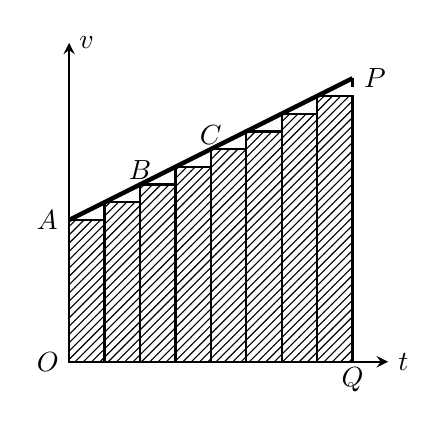
\begin{tikzpicture}[>=stealth, thick,scale=0.9]
  \draw [<->](0,4.5)node [right]{$v$}--(0,0)node [left]{$O$}--(4.5,0)node [right]{$t$};
  \draw [ultra thick] (0,2)node [left]{$A$}--(4,4)node [right]{$P$};
  \draw [dashed](4,4)--(4,0);
  \foreach \x in {1,2,3,4,...,8}
  {
     \fill [pattern = north east lines, draw] (\x/2-.5, 0) rectangle (\x/2, 1.75+\x/4);
  }
  \node at (4,-.25){$Q$};
  \node at (1,2.7){$B$}; 
  \node at (2,3.2){$C$};
\end{tikzpicture}
\end{document}